\subsection[The Naïve string-matching algorithm]{The Naïve string-matching algorithm (Brute-Force approach)}
    \subsubsection{Introduction \& Application}
        %aabccab
        abc
    \subsubsection{Pseudocode}
        \textbf{Notation:}
        \begin{itemize}
            \item \textbf{Text $T$ (R rows, C columns)}: The main text being searched.
            \item \textbf{Pattern $P$ (K the number of keywords)}: The list of strings that we are looking for.
            \item \textbf{Positions ([(start position, end position), \ldots])}: A list storing the indices where a complete match is found.
        \end{itemize}
        \textsc{Brute-Force-2D-Matcher}($T, P, K, R, C$)
        \begin{algorithmic}[1]
        \State $pos = \text{empty array of size } K$
        \For{$idx = 1$ \textbf{to} $K$}
            \State $keyword = P[idx]$
            \State $m = keyword.length$
            \Statex
            \Statex
            \Comment{Search Horizontally}
            \For{$i = 1$ \textbf{to} $R$}
                \For{$j = 0$ \textbf{to} $C - m$}
                    \If{$keyword[1 \dots m] == T[i, j+1 \dots j+m]$}
                        \State \text{add } $position$ \text{ to } $pos[idx]$
                    \EndIf
                \EndFor
            \EndFor
            \Statex
            \Statex
            \Comment{Search Vertically}
            \For{$i = 1$ \textbf{to} $C$}
                \For{$j = 0$ \textbf{to} $R - m$}
                    \If{$keyword[1 \dots m] == T[j+1 \dots j+m, i]$}
                        \State \text{add } $position$ \text{ to } $pos[idx]$
                    \EndIf
                \EndFor
            \EndFor
        \EndFor
        \State \Return $pos$
        \end{algorithmic}
    \newpage
    \subsubsection{Step-by-step trace}
    \indent \textbf{Notation:}
        \begin{itemize}
            \item \textbf{Text $T$ (length $n$)}: The main text being searched.
            \item \textbf{Pattern $P$}: The string that we are looking for.
            \item \textbf{Shift ($s$)}: The current offset of the text T.
            \item \textbf{Positions ([(start position, end position), \ldots])}: A list storing the indices where a complete match is found.
        \end{itemize}

    \indent \textbf{Example:} text $T = [a, a, b, c, a, b, b]$ and pattern $P = [a, b, c]$
    \begin{itemize}
        \begin{figure}[H]
            \centering
            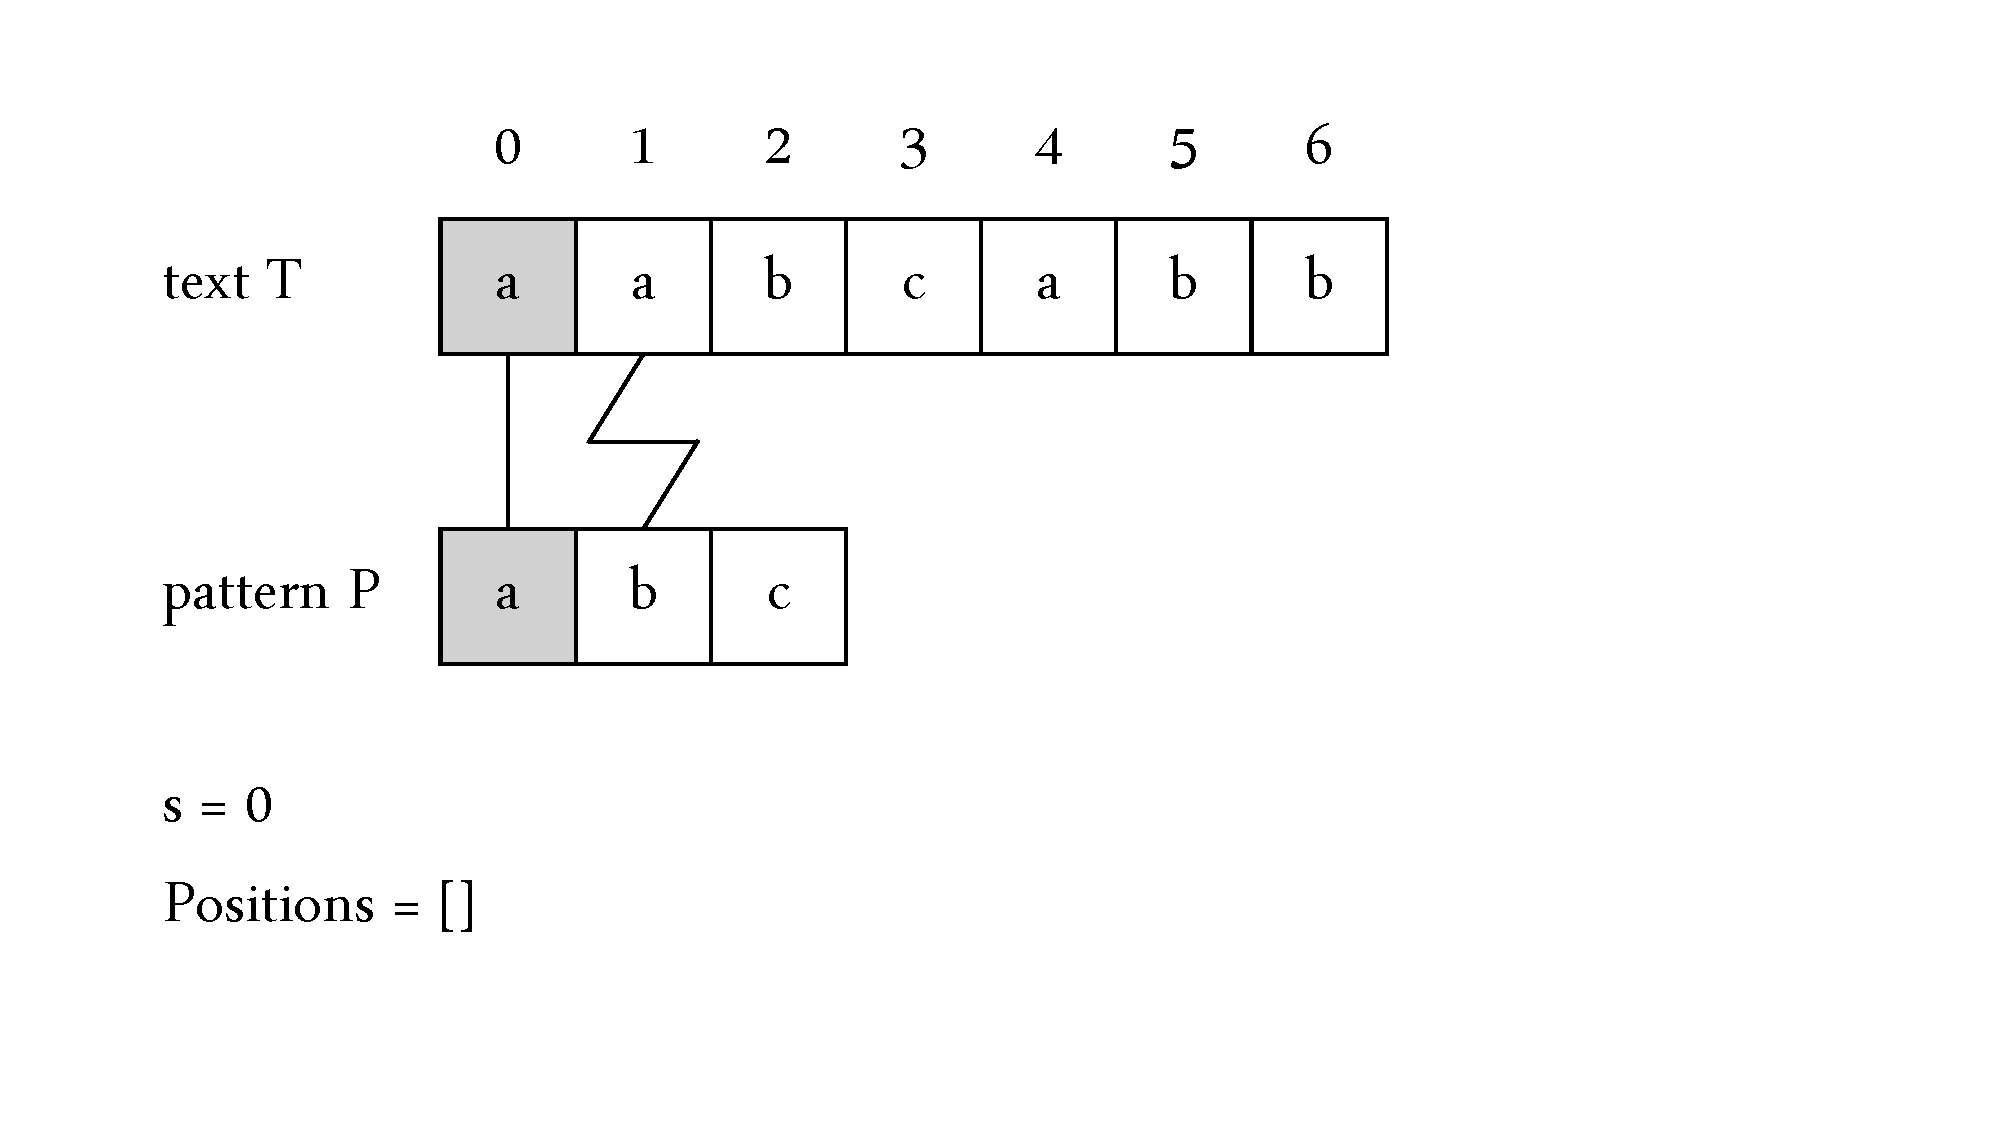
\includegraphics[width=0.8\textwidth, trim={2cm 2cm 5cm 2cm}, clip]{data/Illustrations/brute-force1.pdf}
            \caption{Step 1}
        \end{figure}
        \item The first character 'a' matches in both arrays.
        
        The second character in text T ('a') does not match the second character in pattern P ('b').
        
        Text at the bottom shows the current shift is s = 0 and the list of found matches is empty (Positions = []).
        
        \begin{figure}[H]
            \centering
            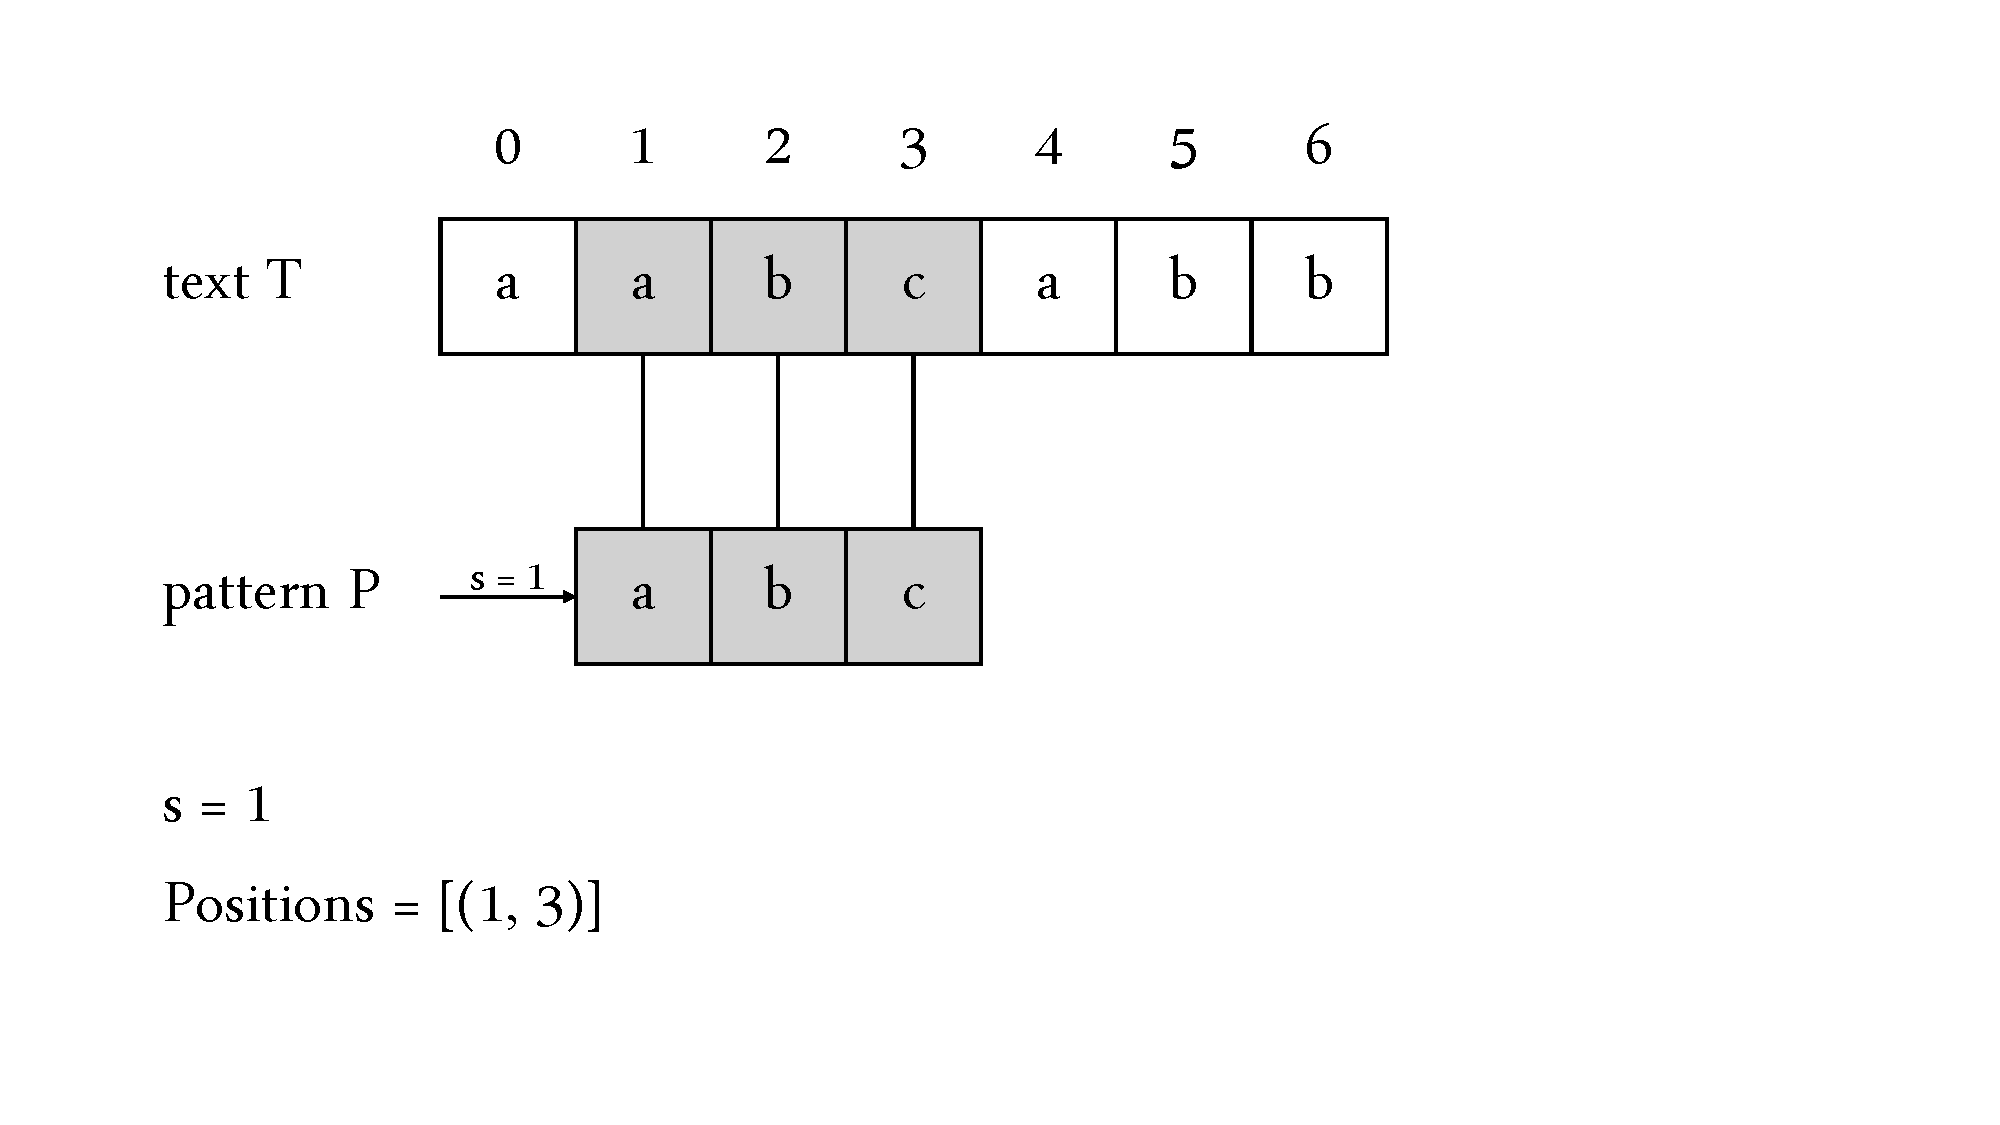
\includegraphics[width=0.8\textwidth, trim={2cm 2cm 5cm 2cm}, clip]{data/Illustrations/brute-force2.pdf}
            \caption{Step 2}
        \end{figure}
        \item All characters in pattern P ('a', 'b', 'c') successfully match the corresponding characters in text T ('a', 'b', 'c').
        
        Shift is s = 1 and the list of found matches is updated to record this position (Positions = [(1, 3)]).

        \begin{figure}[H]
            \centering
            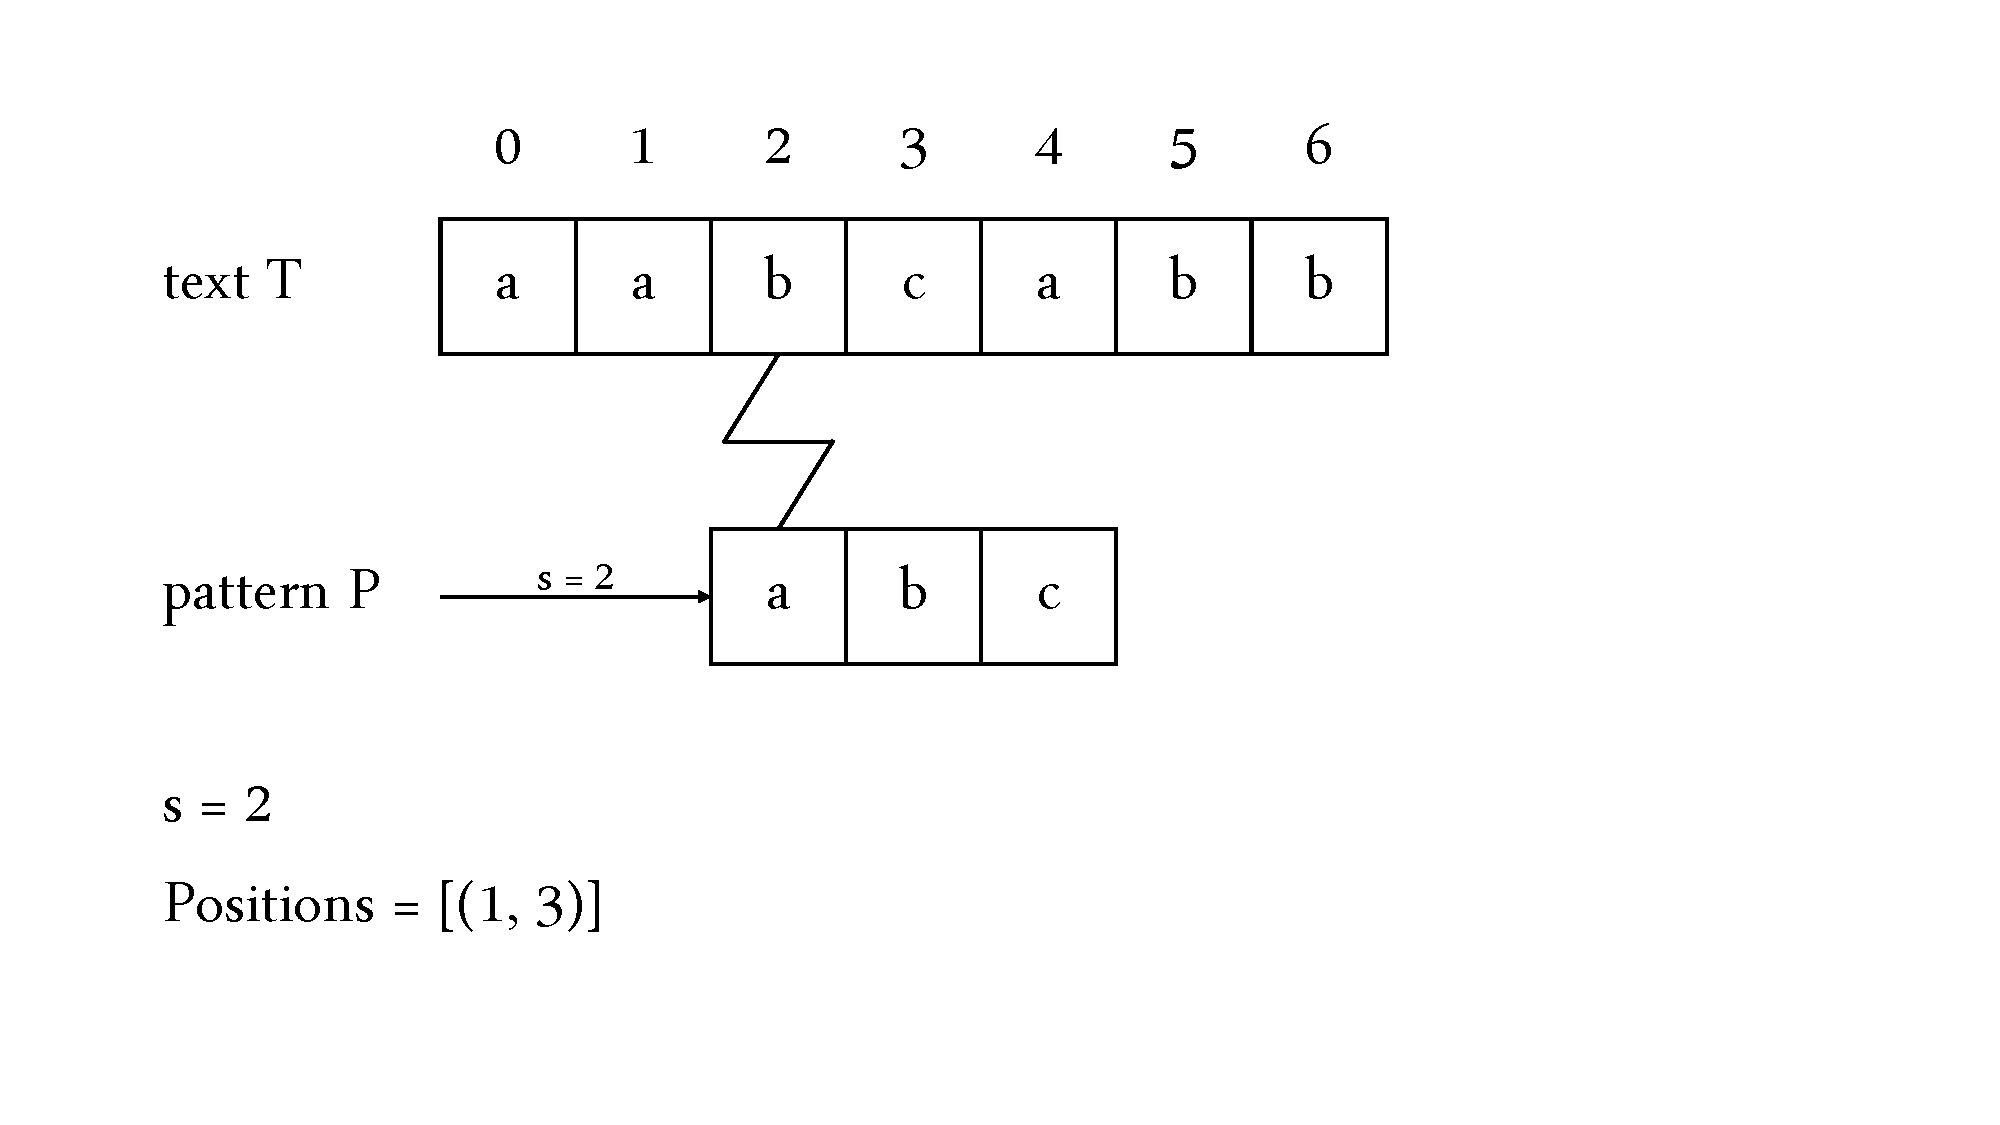
\includegraphics[width=0.8\textwidth, trim={2cm 2cm 5cm 2cm}, clip]{data/Illustrations/brute-force3.pdf}
            \caption{Step 3}
        \end{figure}
        \item The first character in pattern P ('a') does not match the character in text T ('b') at the current shift position s = 2.
        
        Skip to the next shift without updating Positions.

        \begin{figure}[H]
            \centering
            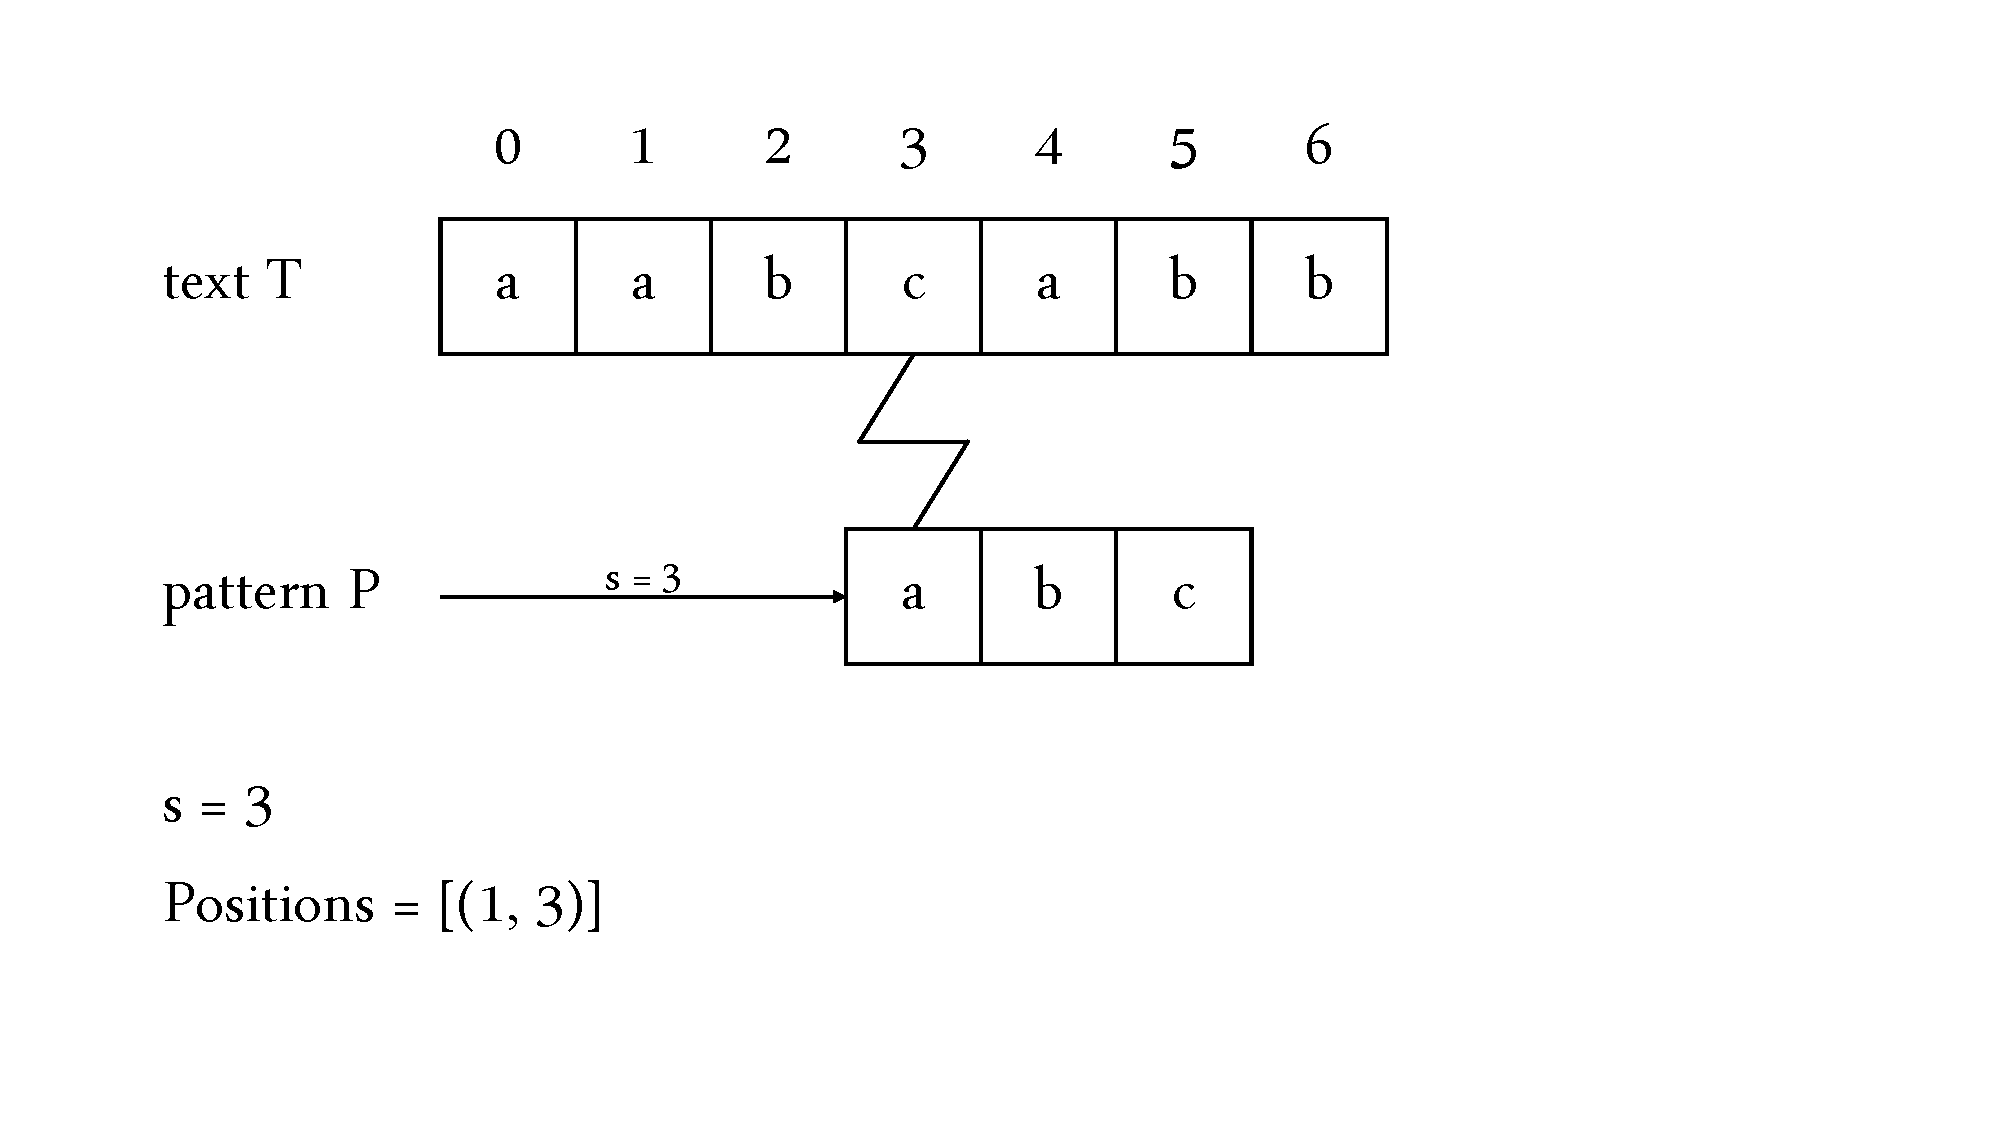
\includegraphics[width=0.8\textwidth, trim={2cm 2cm 5cm 2cm}, clip]{data/Illustrations/brute-force4.pdf}
            \caption{Step 4}
        \end{figure}
        \item The first character in pattern P ('a') does not match the character in text T ('c') at the current shift position s = 2.
        
        Skip to the next shift without updating Positions.

        \begin{figure}[H]
            \centering
            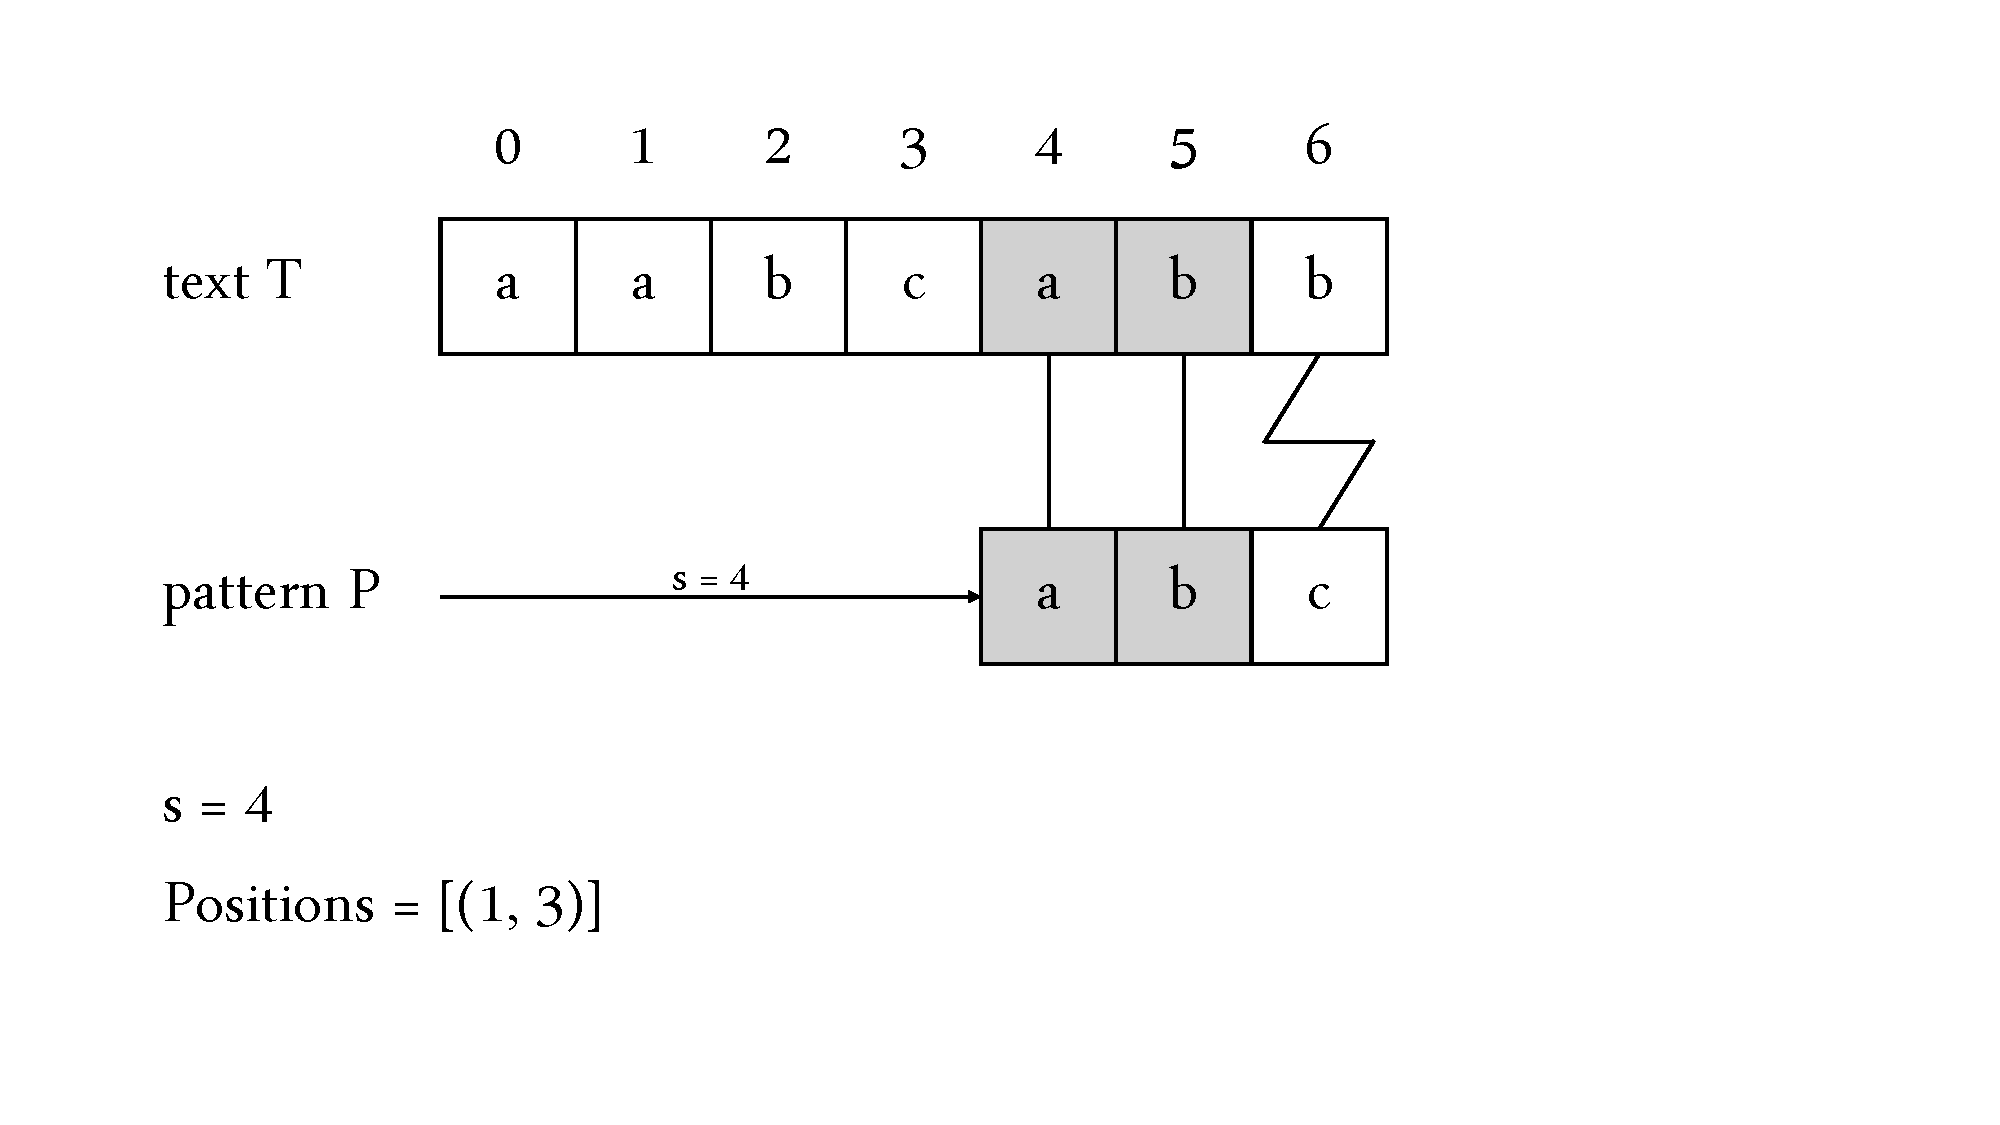
\includegraphics[width=0.8\textwidth, trim={2cm 2cm 5cm 2cm}, clip]{data/Illustrations/brute-force5.pdf}
            \caption{Step 5}
        \end{figure}

        \item The first two characters in pattern P ('a', 'b') match the corresponding characters in text T,
        but the third character in pattern P ('c') does not match the character in text T ('b') at the current shift position s = 4.

        Skip to the next shift without updating Positions.

        \item After that, $s$ increases by 1.Because $s = 5$ and $n - m = 7 - 3 = 4$, we have $s > n - m$. The algorithm terminates and returns the list of found matches: $\text{Positions} = [(1, 3)]$.
    \end{itemize}
    

    \subsubsection{Complexity}
        \begin{table}[H]
        \centering
        \renewcommand{\arraystretch}{1.5}
        \begin{tabular}{|l|c|p{8cm}|}
        \hline
        \textbf{Metric} & \textbf{Complexity} & \textbf{Reasoning} \\ \hline
        \textbf{Time (Worst)} & $O(K \cdot m \cdot R \cdot C)$ & Occurs when patterns and text share many prefix characters (e.g., all 'A's). \\ \hline
        \textbf{Time (Average)} & $O(K \cdot R \cdot C)$ & In practice, a mismatch usually occurs after only a few character comparisons. \\ \hline
        \textbf{Time (Best)} & $O(K \cdot R \cdot C)$ & The first character of the pattern always results in a mismatch at every shift. \\ \hline
        \textbf{Auxiliary Space} & $O(1)$ & The algorithm uses only a constant amount of extra memory for loop indices. \\ \hline
        \end{tabular}
        \caption{Complexity Analysis of 2D Brute Force Algorithm}
        \end{table}


        
    \subsubsection{Discussion}
        